\documentclass[12pt,a4paper]{article}
\usepackage[utf8]{inputenc}
\usepackage[russian]{babel}
\usepackage{amsmath}
\usepackage{amsfonts}
\usepackage{amssymb}
\usepackage{graphics}
\usepackage[pdftex]{graphicx}
\usepackage{lscape}
\usepackage{listings}
\usepackage{geometry} % Меняем поля страницы 
\geometry{left=2cm}% левое поле 
\geometry{right=1.5cm}% правое поле 
\geometry{top=2cm}% верхнее поле 
\geometry{bottom=15mm}% нижнее поле
\renewcommand{\baselinestretch}{1.5}
\pagestyle{plain}
\begin{document}
\thispagestyle{empty}
\begin{center}
\large Санкт-Петербургский государственный политехнический университет\\
Институт информационных технологий и управления\\
Кафедра компьютерных систем и программных технологий\\
\vspace{65mm}
\Large Отчёт по лабораторной работе №1\\ По предмету "Проектирование ОС и компонентов" \\на тему:\\
\LARGE\textbf{Создание инсталлятора для Linux дистрибутива}
\end{center}

\vspace{40mm}
\begin{flushright}
\large Выполнила: студентка группы 53501/3\\ Тарасова А. А.\\ Преподаватель: Душутина Е. В.
\end{flushright}
\vspace{30mm}

\begin{center}
Санкт-Петербург\\ 2015
\end{center} % это титульный лист
\newpage
\tableofcontents
\newpage
Проанализировать инсталляцию ОС Linux,сформировать инсталлятор с минимальным набором функций. В системный редактор всего этого написать command file необходимого сброса. Можно  из оболочки user mode или свой вариант, который сделать сборку. Описание есть у  Fedora.

Вначале спрашивают язык. Выбираем русский.
\begin{figure}[h!]
\centering
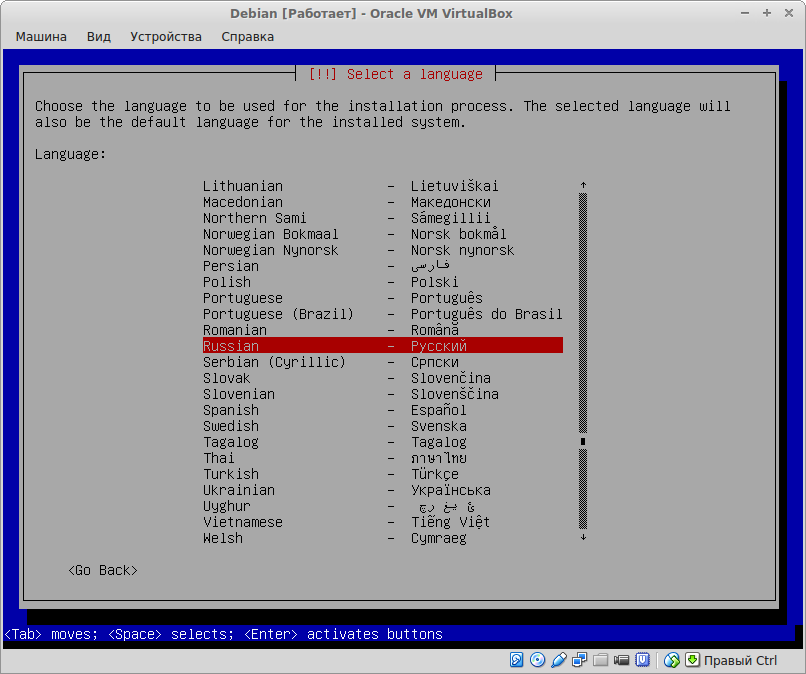
\includegraphics[scale=0.45]{res/russian}
\end{figure}
\section{Разметить диск}
\section{Поднять сеть}
\section{Поставить пакеты}
\section{Первичные настройки}

\end{document}